\section{Ballistisches Pendel}\label{kap:Bal}
\subsection*{Beobachtung und Analyse}
Beobachtet wurde das bei Auslenkung der kleinen Kugel die große Kugel erwartungsgemäß im Vergleich zur Auslenkung der kleinen Kugel bei Aufprall ausgelenkt wurde während die kleine Kugel beim Zusammenstoß mit der kleinen Kugel deutlich stärker ausgelenkt wurde als die große Kugel.

\begin{figure}[h]
	\centering
	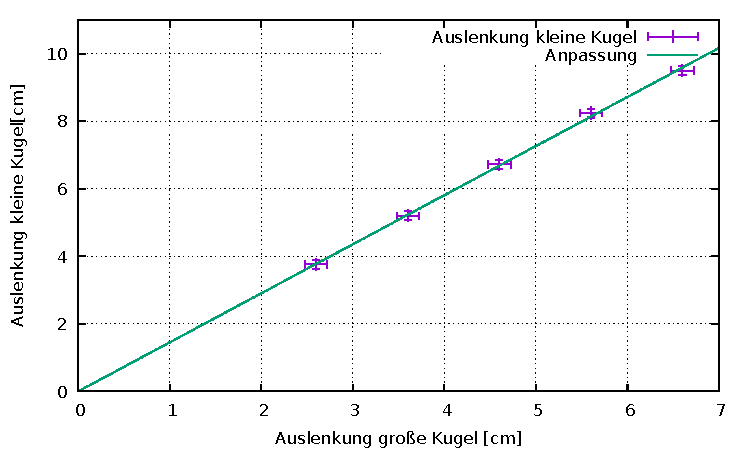
\includegraphics[width=0.8\textwidth]{res/GrosKlein.pdf}
	\caption{Zu sehen ist die Auslenkung der kleinen Kugel in Abhängigkeit von der Auslenkung der großen Kugel.}
	\label{fig:grosklein}
\end{figure}
\begin{figure}[h]
	\centering
	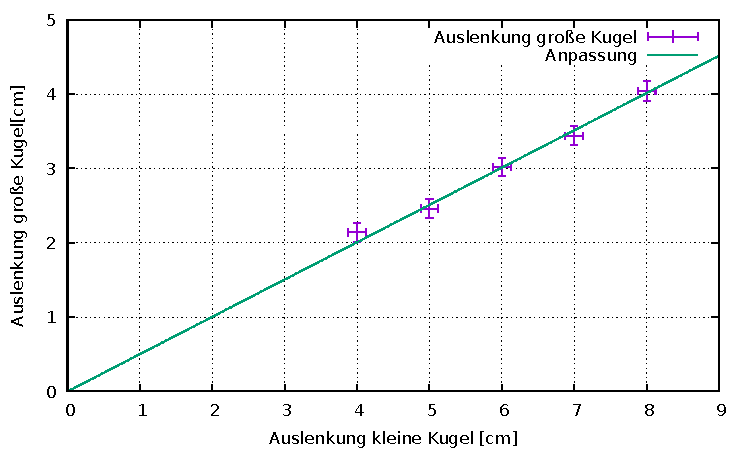
\includegraphics[width=0.8\textwidth]{res/KleinGros.pdf}
	\caption{Zu sehen ist die Auslenkung der großen Kugel in Abhängigkeit von der Auslenkung der kleinen Kugel.}
	\label{fig:kleingros}
\end{figure}

Die bei den fünf Messreihen erhaltenen Messwerte wurden jeweils gemittelt und sind in den Abbildungen \ref{fig:grosklein} und \ref{fig:kleingros} zu sehen. Die Fehlerbalken Ergeben sich aus den Gleichungen \ref{eq:sud}, \ref{eq:sunv} und \ref{eq:kombsu}. 
Man erkennt das die Messwerte linear ansteigen. Da dies mit der Theorie übereinstimmt (Die Auslenkung nach dem Stoß ist durch
\begin{align}
	a_2= \frac{2m_1}{m_1+m_2} a_1\label{eq:Auslenkung}
\end{align} 
gegeben wobei $m_1$ die Masse der ausgelenkten Kugel ist und $a_1$ die Auslenkung von $m_1$)
wurden die Messwerte mit der Linearen Anpassung\footnotetext{Die Anpassung wurde durch „Gnuplot“ mit dem Levenberg–Marquardt Algorithmus vorgenommen.} $a_2=b*a_1$)angepasst.Und die Unsicherheit der Anpassung wurde aus Gnuplot entnommen.
Um die Ergebnisse zu überprüfen wurde die Steigung $b$ aus den Massen der Kugeln bestimmt. Die Unsicherheit der Masse, ist durch die Anzeigeungenauigkeit der Digitalen Waage, die auf zwei Nachkommastellen genau anzeigt, gegeben. Und somit folgt mit den Gleichungen \ref{eq:sur} und \ref{eq:kombsu}. Der Vergleich der Werte ist in Tabelle \ref{tab:steigung} zu sehen.
Man erkennt das die Werte zwar voneinander Abweichen jedoch nur um ca. $3\%$ (Groß gegen Klein) bzw. um ca. $2\%$ (Klein gegen Groß). Dies ist darauf zurückzuführen das es sich bei dem Untersuchten Stoß nicht um einen perfekten elastischen Stoß handelte bzw. das die Pendel nicht immer tatsächlich vollkommen ruhig hingen.
Über das Verhältnis der Steigungen der Anpassungsfunktion erhält man ein auch das Gewichtsverhältnis, dass sich über: 
\begin{align}
\frac{b_1}{b_2}=\frac{m_1}{m_2}	
\end{align} 
($b_1$, $m_1$ Steigung bzw. ausgelenktes Gewicht aus Abb. \ref{fig:grosklein} und $b_2$,$m_3$ Steigung bzw ausgelenktes Gewicht aus Abb. \ref{fig:kleingros} ) berechnen lässt. die Ergebnisse sind in Tabelle \ref{tab:Gewicht} zu sehen.
Man sieht das das aus den Massen berechnete Gewichtsverhältnis  noch innerhalb der Unsicherheit des aus den Steigungen berechneten Verhältnisses liegt. Dies lässt darauf schließen, dass dieses verfahren recht genau ist.

\begin{table}[h]
	\begin{tabular}{|c|c|c|}
		\hline
		& Steigung Theoretisch & Steigung Experimentell\\
		& bestimmt & bestimmt\\
		\hline
		Groß gegen Klein &  \SI{1,487+-0,0002}{} & \SI{1,453+-0,016}{} \\
		\hline
		Klein gegen Groß & $0,513 \pm 6 \cdot 10^{-5}$&\SI{0,502+-0,006}{}\\
		\hline
	\end{tabular}
\caption{Zu sehen sind die Steigungen der in Abb. \ref{fig:grosklein} und \ref{fig:kleingros} zu sehenden Anpassungsgeraden.}
\label{tab:steigung}
\end{table}
\begin{table}[h]
	\begin{tabular}{|c|c|}
		\hline
		Gewichtsverhätnis aus  & Gewichtsverhältnis aus\\
		 den Gewichten & der Steigung\\
		\hline
		$0,3451 \pm 6 \cdot 10^{-6}$& \SI{0,3455+-0,004}{}\\
		\hline
	\end{tabular}
	\caption{Zu sehen ist hier das Gewichtsverhältnis der Kleinen Kugel zur Großen Kugel.}
	\label{tab:Gewicht}
\end{table}
